
%(BEGIN_QUESTION)
% Copyright 2006, Tony R. Kuphaldt, released under the Creative Commons Attribution License (v 1.0)
% This means you may do almost anything with this work of mine, so long as you give me proper credit

A water reservoir located high on a hill stores fresh water for a town's drinking needs.  A float connected to a lever provides visual indication of the water level inside the reservoir.  Nearby this reservoir, a person has the most boring job in the world: to turn the pump on when the water level gets too low, and to turn the pump off when the water level gets too high.  Note that the float mechanism showing water level in the reservoir cannot show the entire capacity of the reservoir, but only the top ten feet (from 20 feet to 30 feet of level):

$$\includegraphics[width=15.5cm]{i00080x01.eps}$$

As crude as it is, this system contains {\it instrumentation}, and we may apply standard instrumentation terms to its components.  Apply the following terms to this water-supply system, as best as you can:

\begin{itemize}
\item{} Process
\item{} Primary sensing element
\item{} Final control element
\item{} Measurement range
\item{} Lower-Range Value (LRV)
\item{} Upper-Range Value (URV)
\item{} Measurement span
\item{} Indicator
\item{} Transmitter
\item{} Controller
\item{} Measured Variable (or Process Variable)
\item{} Controlled Variable (or Manipulated Variable)
\end{itemize}

\underbar{file i00080}
%(END_QUESTION)





%(BEGIN_ANSWER)

\begin{itemize}
\item{} Process: {\it the water and all associated vessels, pipes, and pump}
\item{} Primary sensing element: {\it float}
\item{} Final control element: {\it pump}
\item{} Measurement range: {\it 20 ft to 30 ft}
\item{} Lower-Range Value (LRV): {\it 20 ft}
\item{} Upper-Range Value (URV): {\it 30 ft}
\item{} Measurement span: {\it 10 ft}
\item{} Indicator: {\it pointer and scale}
\item{} Transmitter: {\it lever, fulcrum, and cables}
\item{} Controller: {\it bored person}
\item{} Measured Variable (or Process Variable): {\it water level}
\item{} Controlled Variable (or Manipulated Variable): {\it pump speed (on/off status)}
\end{itemize}

The distinction between measurement range, LRV, URV, and span is important.  What we are measuring here is water level in the tank between the 20 and 30 foot marks.  The difference in level between these marks is what we call the {\it span}.  So in this case we have a span of 10 feet (30 feet $-$ 20 feet).  The LRV is the lower end of the measurement range: 20 feet.  The URV is the upper end of the measurement range: 30 feet.  The {\it range} of measurement encompasses both LRV and URV, and is stated ``20 to 30 feet''.

By the same token, if you had a pressure transmitter in an air separation process ranged from 200 to 500 PSI, 200 PSI would be the LRV, 500 PSI would be the URV, and 300 PSI would be the span.

\vskip 10pt

In any instrument system, the {\it controller} is the thing making control decisions.  In this particular case, it would be the bored person.  All the other hardware between the float and indicating pointer simply transmits information from the reservoir to that bored person (controller).

\vskip 10pt

For the record, I really despise the term ``controlled variable''.  I find it misleading and confusing, but unfortunately it is often used when discussing process controls.  While the ``measured'' or ``process'' variable is the thing we are measuring (and trying to hold to setpoint), the ``controlled'' or ``manipulated'' variable is the thing we are adjusting to effect the process variable.  In this case, the process variable is the water level in the reservoir, and the controlled (or manipulated) variable is the pump speed.  We are measuring water level, and controlling it by turning the pump on and off.

By analogy, imagine a cruise-control system in a car.  The measured (process) variable there is car speed, while the accelerator pedal position is the controlled or manipulated variable, because pedal position is the variable adjusted by the cruise control system in order to maintain the car's speed at setpoint.

Here are some generalized definitions:

\begin{itemize}
\item{} Measured Variable (or Process Variable): {\it The variable we are measuring, usually with intent to hold to a constant setpoint value}
\vskip 5pt
\item{} Controlled Variable (or Manipulated Variable): {\it The variable directly manipulated by the controller, which effects the process variable}
\end{itemize}


%(END_ANSWER)





%(BEGIN_NOTES)


%INDEX% Basics: water reservoir level control system
%INDEX% Process: municipal water storage tank

%(END_NOTES)


